
\section{The Sugarscape in its Original Implementation}

A famous agent-based model is Epstein and Axtell’s “Sugarscape,” explained in detail in their book \underline{Growing Artificial Societies}. Sugarscape is a virtual 2D grid where each cell has a certain amount of “sugar” or “spice” that increases at a certain rate. Agents roam the grid, consuming sugar as they visit cells.

In the simplest Sugarscape, each agent has a sugar reserve, a metabolism at which rate it consumes its sugar, and a range of nearby cells that it can observe. At each time step, the agent observes its nearby cells and moves to the cell with the most sugar. These rules can be expanded to include topics as varied as reproduction, death, disease, loans, and warfare. For example, a disease can be introduced to the system where any sick agent can infect nearby healthy agents without immunity.

Despite its simplicity, the model shows emergent behavior that resembles the real world. When modeling wealth with Sugarscape, a long tailed distribution appears where some agents are exponentially richer than others. This complex behavior is seen in the United States, where wealth is a Pareto distribution with the top 20\% owning about 85\% of the total wealth. In general, a long tailed distribution is viewed as a negative because it means there are many people barely surviving while others are fabulously rich. 

\section{\#Occupy}

Wealth inequality has partly fueled a modern social movement known as “Occupy”. The first significant Occupy protest was on Wall Street, where thousands of protesters gathered to express their dismay against the wealth distribution, among other things. The movement's motto is “We are the 99\%”, reminding politicians to serve the majority, not the 1\% who control more than a third of the nation's wealth. A major goal of the movement is to achieve a more equal distribution of income, which protesters hope to accomplish by implementing a more progressive tax policy. 

There is little debate about the fact that taxes redistribute wealth from the rich to the poor. What opponents of the Occupy movement (and fiscal conservatives in general) claim is that high tax rates for the rich actually hurt the population as a whole. The logic is that wealthy people employ the poor, redistributing the wealth without the need for tax levies. 

\section{A New Take on Sugarscape}

Our implementation of Sugarscape aims to study the effect of taxation on the wealth of a society. We want to show how extreme under or over taxation can affect the society and its individual agents, and what happens in between these two extremes. The model tests a “flat tax” system where every agent gets taxed a constant rate (say 10\% of its total wealth) and the tax pool is redistributed evenly among all the agents. We recreate the original Sugarscape and expand on it with the end goal of determining if it is possible to shrink the wealth gap without crippling the society.

\subsection{Pygame}

In the process of implementing Sugarscape, we made a GUI to better understand what was happening on the grid. The visualization of the Sugarscape is done with Pygame, a set of Python modules that allows easy graphic drawing. Pygame can ‘blit’ images onto the screen and it has built-in methods for handling user input like mouse clicks and button presses, making it ideal for designing game or other programs that receive a lot of input.

Below is an abbreviated version of our event loop that draws the cells in the GUI at each timestep. Sugarscape.nextstep() moves every agent forward by one timestep and the rest of the code redraws the update. Redrawing the entire grid is slightly less efficient than changing existing rectangle objects but is a common convention for pygame. A square is drawn for each location, and the color of the square changes based on the amount of sugar contained there. Agents are represented by circles drawn on top of their current location.

\begin{verbatim}

  def event_loop(self,sugarscape):
   while True:
    sugarscape.nextstep()
    for i in range(sugarscape.length):
     for j in range(sugarscape.width):
      loc=sugarscape.get_location(i,j)
      health_color=(0, 0,loc.get_sugar_amt()/loc.get_max_sugar())
      pygame.draw.rect(self.window,healthColor,(12*i,12*j,10,10))
    pygame.display.update()
\end{verbatim}

Users can control certain attributes of the Sugarscape by moving sliders underneath the grid. A histogram, implemented using the matplotlib library, shows the current distribution of wealth, and text fields show certain characteristics of the distribution. 

\section{Taxation and the Leave Behind}

Taxation in our implementation of Sugarscape is handled with a “Government” object. Every ten timesteps, the Government object collects a constant percentage of each agent's sugar reserve. The Government then immediately redistributes the collected sugar to each agent equally.

Taxation is a novel concept in Sugarscape, but the implementation described above does not fully capture a society's response to taxation. In a real society, the wealthiest contribute to society more than the poor because they can open factories, do research and development, and generally make investments into the economy. In order to simulate the benefits that a few wealthy people bring into an economy, we need to implement some mechanism for the rich to contribute more to a society than the poor. As such, we implement a simple “leave behind” feature, where agents leave some sugar behind as they leave a location. The amount that they leave behind is calculated:

$sugar = \frac{wealth\times N}{total\_wealth}^{1.1} \times \frac{1}{5}$

where N is the total number of agents, wealth is the amount of sugar the agent currently has, and total wealth is the total amount of sugar owned by all the agents. Agents who own a large proportion of the total wealth leave behind larger amounts of sugar, making an “investment” into the Sugarscape, and creating wealth around it. 

\subsection{What is a Gini coefficient?}

In order to compare tax rates objectively based on their wealth distribution, we need a metric that can measure how distributed or flat a certain wealth distribution is. We use the Gini coefficient, which is often used in economics to measure the wealth gap (named after Corrado Gini who developed it in 1912). This coefficient allows us measure how well the wealth is distributed. The value is always between 0 and 1, with 0 the measurement of a perfectly uniform distribution, and 1 the measurement of a distribution with complete inequality.

A good way to visualize Gini coefficients is a Lorenz curve.  A society's wealth inequality is visualized by the curvature of the graph, where a perfectly distributed society is a straight line.

\begin{figure}[h!]
\centering
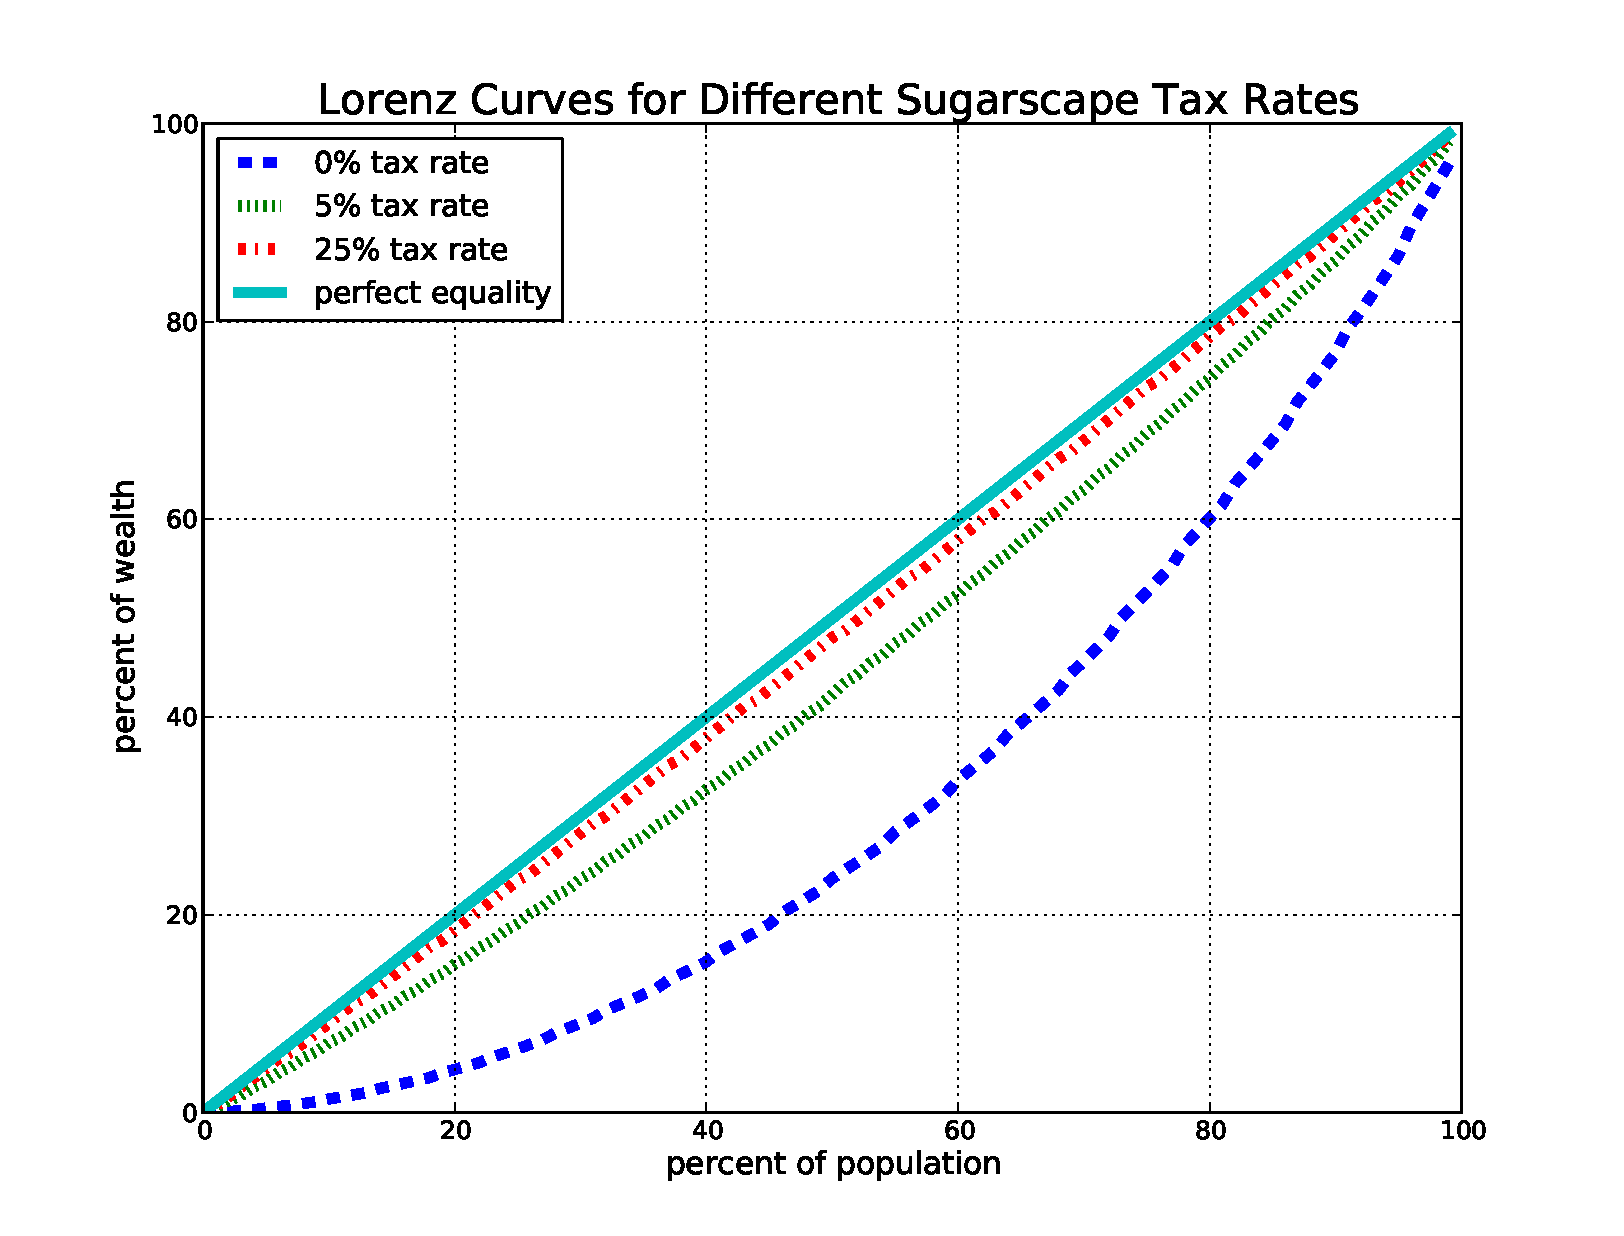
\includegraphics[scale=.4]{case_studies/sugarscape/lorenz.pdf}
\caption{Lorenz curves for different tax rates.}
\end{figure}

\subsection{Results Without Taxation}

\begin{figure}[h!]
\centering
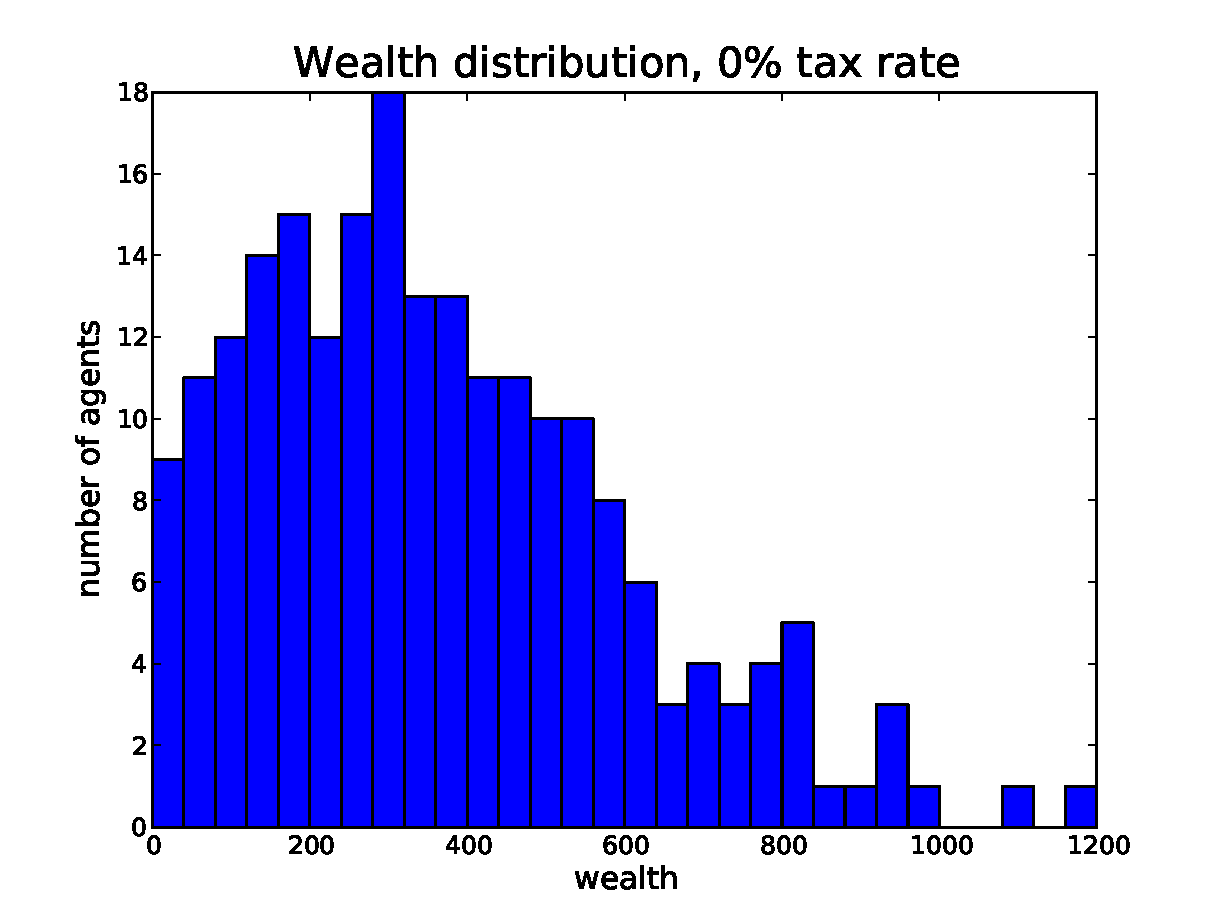
\includegraphics[scale=.5]{case_studies/sugarscape/pmf_notax.pdf}
\caption{PMF with no tax.}
\end{figure}

Figure 3 shows a histogram describing the wealth distribution when there is no tax system in place. For most initial conditions without taxation, the Sugarscape quickly develops a long-tailed distribution of wealth, skewed to the right. In these cases, some agents die quickly, particularly in an environment with many agents or one with low sugar regrowth rate. The separation between the rich and the poor is significant, and there aren't many agents occupying the middle ground. This is seen in real life in societies where there is no tax structure and there isn't much of a middle class.

\subsection{Results With Taxation}

\begin{figure}[h!]
\centering
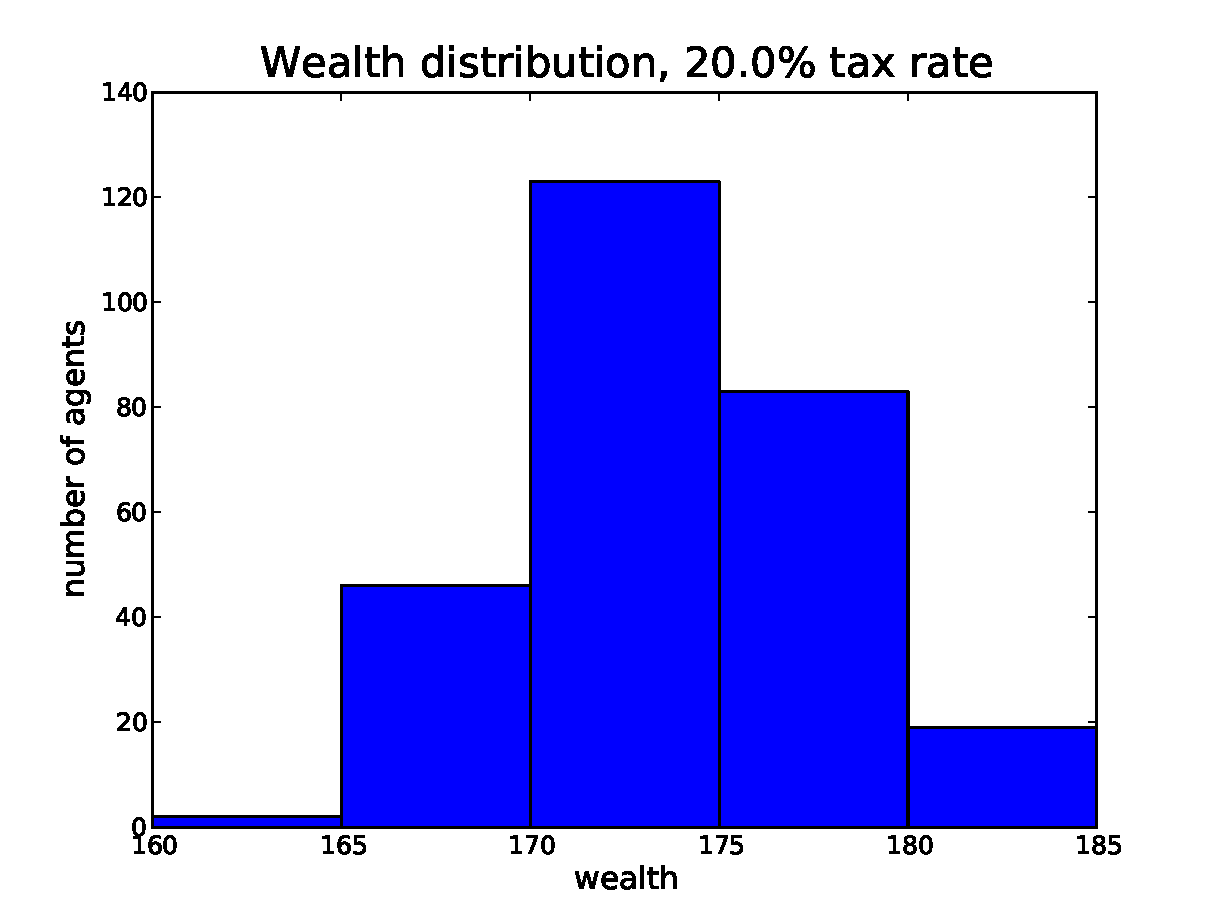
\includegraphics[scale=.5]{case_studies/sugarscape/pmf_20percent.pdf}
\caption{}
\end{figure}

Figure 2 shows our results with a relatively high tax rate. The agents have a similar amount of sugar, and the economy has a very low Gini coefficient (.02). Figure 3 confirms this, showing that higher taxes in general result in lower Gini coefficients. This makes sense, since the point of our tax system is to redistribute the wealth.

One drawback to such a small deviation of wealth is the effect it has on the mean wealth. The mean in figure 2 (with 20\% tax) is 157, compared to the 0\% tax rate case where the mean is 358. Figure 5 shows the plot of the tax rate versus the mean wealth, which shows that the mean wealth gets smaller as taxes get higher.


\begin{figure}[h!]
\centering
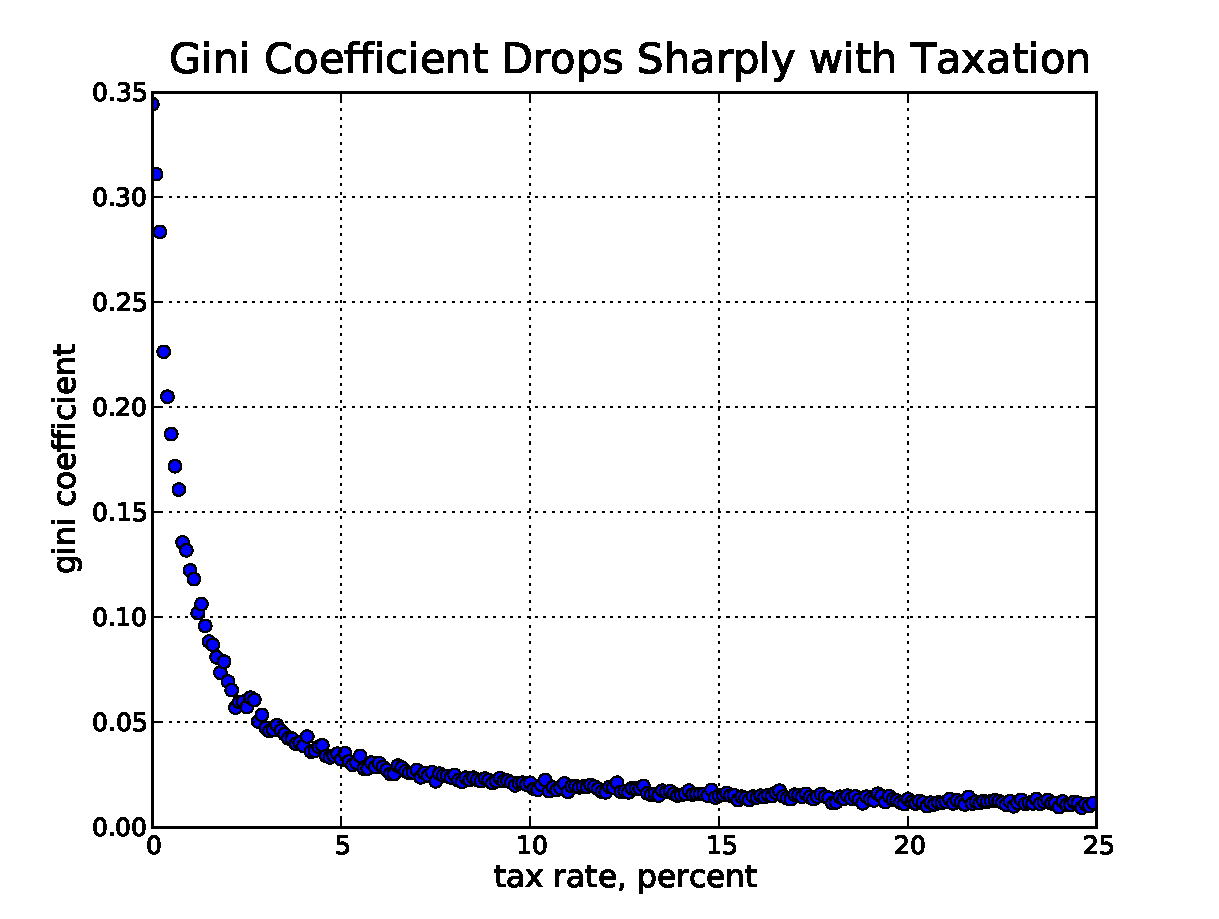
\includegraphics[scale=.5]{case_studies/sugarscape/gini_coeff.pdf}
\caption{The Gini coefficient versus the tax rate.}
\end{figure}

\begin{figure}[h!]
\centering
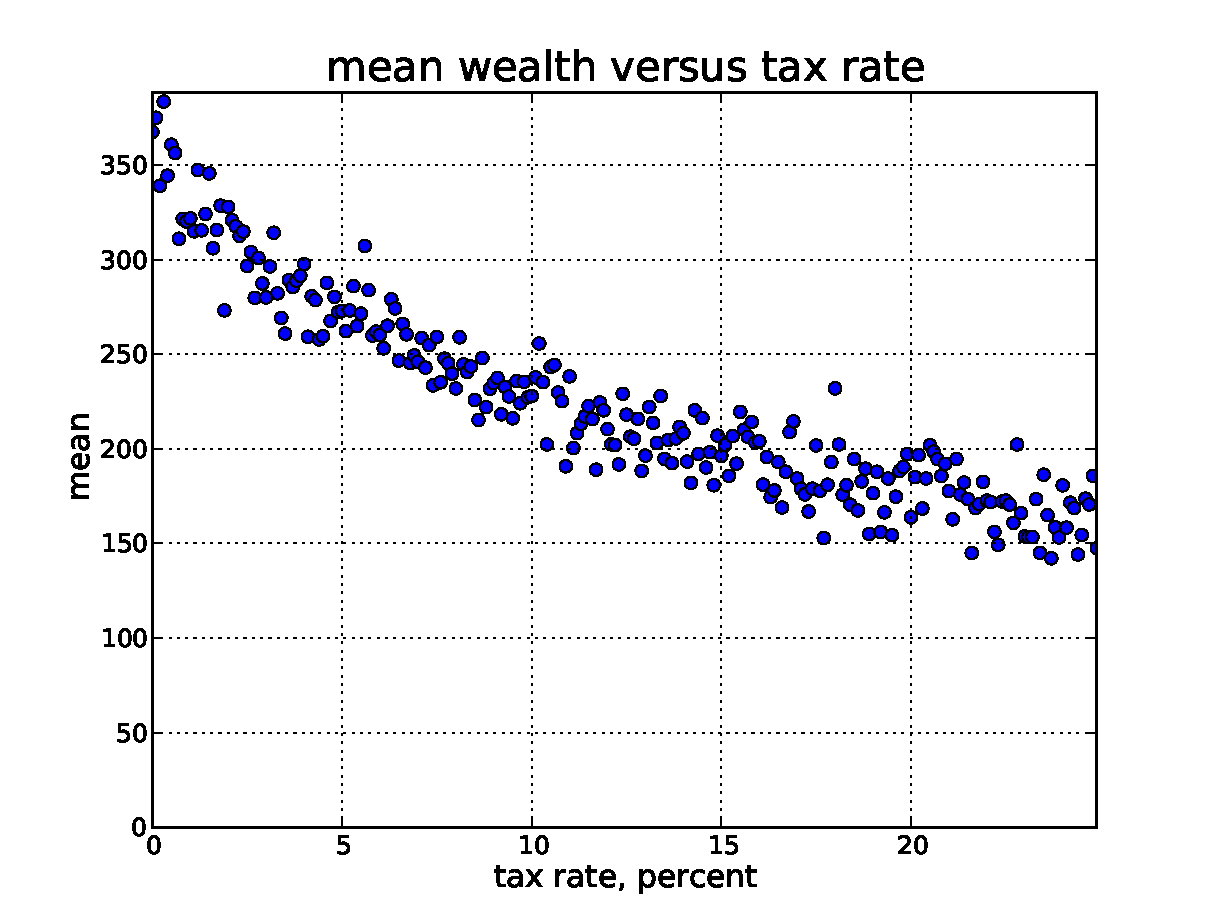
\includegraphics[scale=.5]{case_studies/sugarscape/mean_wealth.pdf}
\caption{The tax rate plotted against the mean wealth of the Sugarscape agents. The mean wealth decreases as the tax rate increases, showing the tax rate's effect on the wealth of the agents.}
\end{figure}


\section{Conclusion}

It's up to a society to determine its ideal wealth distribution. If a society values total wealth above all else, the best way to achieve that is with zero taxation. Figure 4 shows that taxation causes the total wealth in a society to decline. All the way to the left, at zero taxation, is analogous to a purely capitalist system. The other end of the spectrum is a Marxist system with total taxation and even wealth redistribution. The capitalist system produces more total wealth, while a Marxist system does not allow for much variability.

These two systems are at odds with each other, and neither fully represent how a real-world society values wealth. A real society would want as much wealth as possible while still preventing poverty. An effective way to track how the lower class is doing is showing how the bottom quartile’s wealth changes with taxation. In figure 5, we see the average wealth of the bottom quartile reaches a peak around a tax rate of 4\%. 

As the tax rate gets higher, the bottom quartile's wealth initially climbs, which is expected as taxation is designed to aid the poorest in a society. But at a critical point around 3\%, the bottom quartile's wealth drops too--this is the point where the society's decline overcomes the taxation's aid. 

\begin{figure}[h!]
\centering
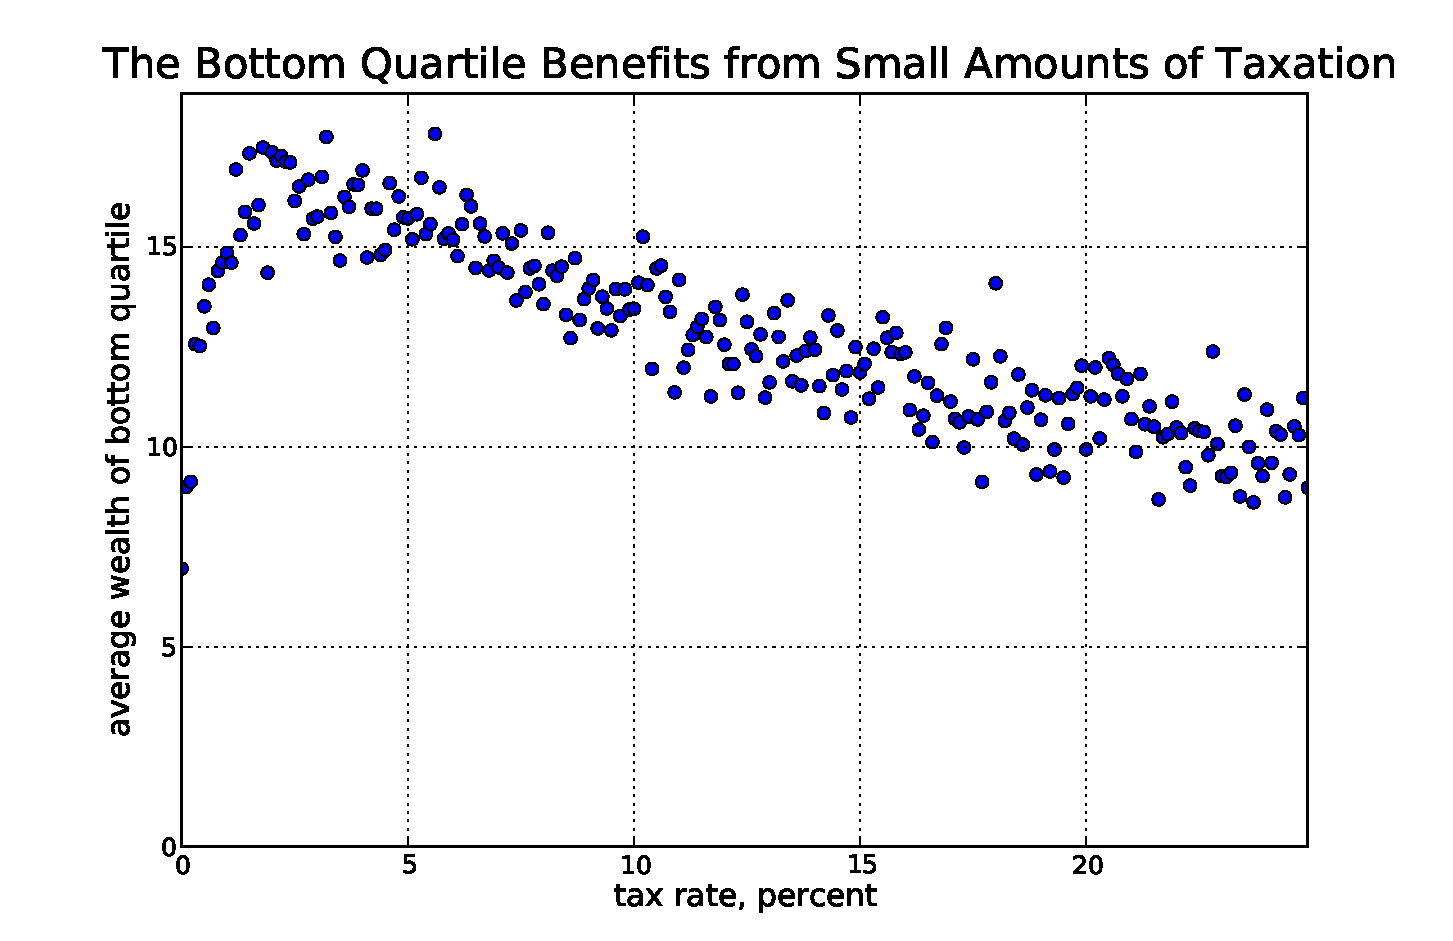
\includegraphics[scale=.45]{case_studies/sugarscape/bottom_quartile.pdf}
\caption{Bottom quartile value versus tax rate. There is a critical point around a tax rate of 4\% where the average wealth of the bottom quartile is maximized.}
\end{figure}


\begin{figure}[h!]
\centering
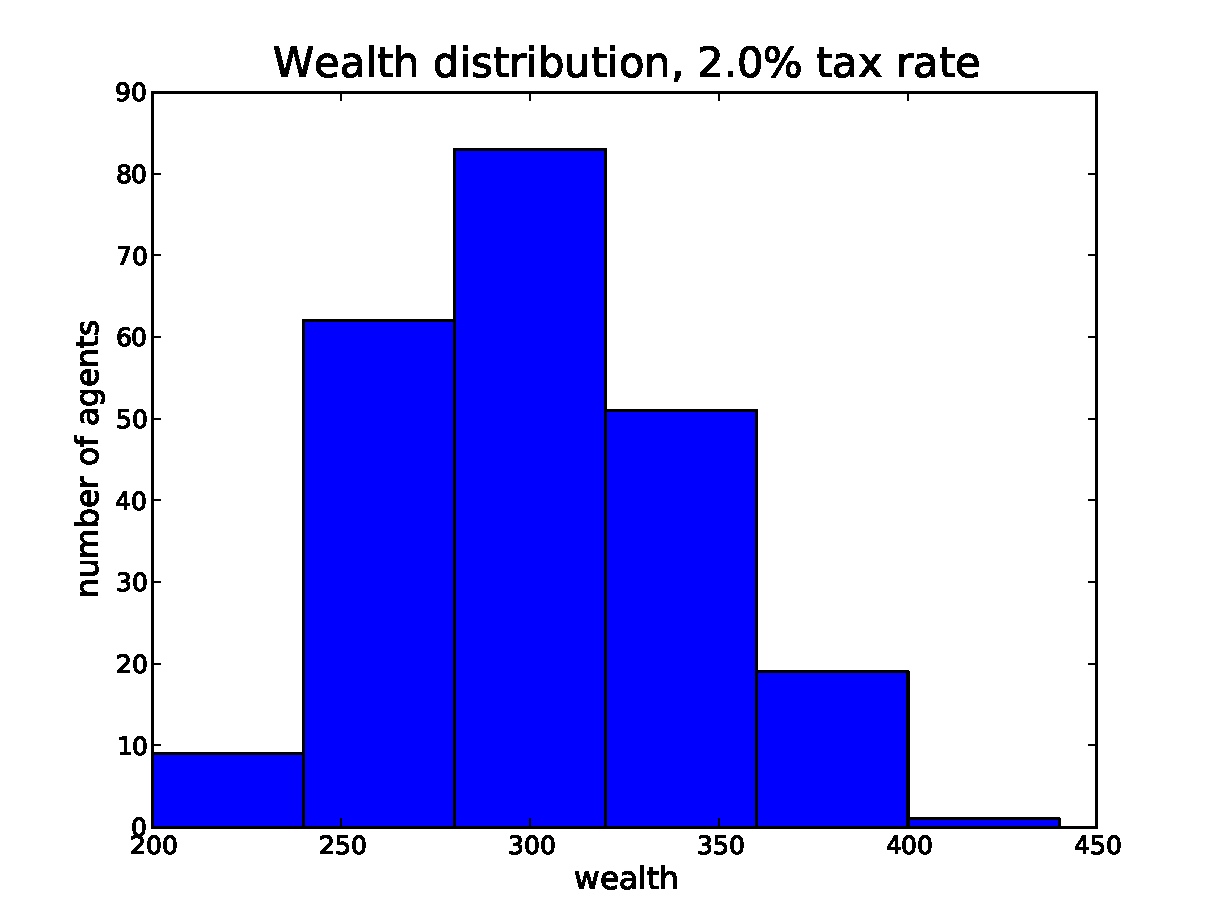
\includegraphics[scale=.5]{case_studies/sugarscape/pmf_2percent.pdf}
\caption{The wealth distribution for a smaller tax rate (2\%). There is still some deviation, but the mean wealth is high.}
\end{figure}

This means, given our Sugarscape, we will minimize our poorest's plight by implementing a 4\% tax. This means that some taxation should be in place to avoid severe poverty, but over-taxation does more harm than good.

Imagining a society's total wealth as a pie helps explain this behavior. In a purely capitalist system, the pie is very large, but some members of society have very small slices. In a purely Marxist system, the pie is small, but everyone shares it equally. The goal of a balanced society is to make the smallest piece of the pie large enough to sustain an acceptable quality of life. 

Our Sugarscape’s taxing implementation showed this trade off in the decreasing trends of the Gini coefficient and mean wealth as the tax rate increases. With higher taxes, there is more wealth, but also more inequality. We have justified a tax rate of 4\% because it results in the highest wealth for the bottom quartile, in effect minimizing poverty in a society.

